\chapter{\sffamily Online simulation inference}

{\bfseries\sffamily Concept.} To extend the formalism that we developed in the previous chapter to describe the time evolution of state probabilities. Having introduced the basic concepts, we then use this formalism to motivate some important methods for probabilistic learning, which we then use in developing a framework for online simulation inference. For the mathematically-inclined, this chapter will take a detailed look at how our formalism can be extended to focus on the time evolution of probabilities, with a view to online simulation inference later on. For the programmers, all of the relevant software lives in this public Git repository: \href{https://github.com/umbralcalc/learndadex}{https://github.com/umbralcalc/learnadex}.

\section{\sffamily Probabilistic formalism} 

This book is about building more realistic training environments for machine learning systems in the real world. In the last chapter we formalised, designed and built a generalised simulation engine which could serve as the essential scaffolding for these environments. So why then, in this chapter, do we want to extend our formalism to talk about probabilistic learning methods?

For many of these realistic environments where only partial state observations are possible, probabilistic learning tools can immediately become an essential tool to robustly infer the state of a system and predict its future states from any given point in time. Given that these tools are often so important for extending the capability of learning algorithms to deal with partially-observed domains; we propose to extend the idea of what is more conventionally considered a `machine learning environment' to include tools for system state inference and future state prediction. In this sense, this chapter, and the remaining chapters of this book, will consider probabilistic learning as an essential part of the environment for a machine learning system.

In this chapter, we're going to begin by discussing the formal connections between some probabilistic learning methods and the simulation formalism we introduced in the last chapter. Let's start by returning to the formalism that we introduced in that chapter. As we discussed at that point; this formalism is appropriate for sampling from nearly every stochastic phenomenon that one can think of. We are going to extend this description to consider what happens to the probability that the state history matrix takes a particular set of values over time.

\begin{figure}[h]
\centering
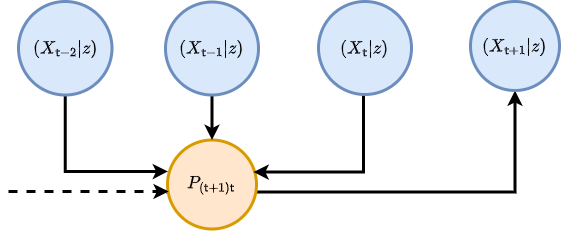
\includegraphics[width=12cm]{images/chapter-2-master-eq-graph.drawio.png}
\caption{Graph representation of Eq.~(\ref{eq:master-x-cont}).}
\label{fig:master-eqn}
\end{figure} 

So, how do we begin? Previously, we defined the general stochastic process with the formula $X^{i}_{{\sf t}+1} = F^{i}_{{\sf t}+1}(X_{0:{\sf t}},z,{\sf t})$. This equation also has an implicit \emph{master equation} associated to it that fully describes the time evolution of the \emph{probability density function} $P_{{\sf t}+1}(X\vert z)$ of $X_{0:{\sf t}+1}=X$ given that the parameters of the process are $z$. This can be written as
%%
\begin{align}
P_{{\sf t}+1}(X\vert z) &= P_{{\sf t}}(X'\vert z) P_{({\sf t}+1){\sf t}}(x\vert X',z) \label{eq:master-x-cont}\,,
\end{align}
%%
where for the time being we are assuming the state space is continuous in each of the matrix elements and $P_{({\sf t}+1){\sf t}}(x\vert X',z)$ is the conditional probability that $X_{{\sf t}+1}=x$ given that $X_{0:{\sf t}}=X'$ at time ${\sf t}$ and the parameters of the process are $z$. To try and understand what Eq.~(\ref{eq:master-x-cont}) is saying, we find it's helpful to think of an iterative relationship between probabilities; each of which is connected by their relative conditional probabilities. We've also illustrated this kind of thinking in Fig.~\ref{fig:master-eqn}.

Consider what happens when we extend the chain of conditional probabilities in Eq.~(\ref{eq:master-x-cont}) back in time by one step. In doing so, we retrieve a joint probability of rows $X_{{\sf t}+1}=x$ and $X_{{\sf t}}=x'$ on the right hand side of the expression 
%%
\begin{align}
P_{{\sf t}+1}(X\vert z) &= P_{{\sf t}-1}(X''\vert z) P_{({\sf t}+1){\sf t}({\sf t}-1)}(x,x'\vert X'',z) \label{eq:master-x-pairwise-joint}\,.
\end{align}
%%
Since Eqs.~(\ref{eq:master-x-cont}) and~(\ref{eq:master-x-pairwise-joint}) are both valid ways to obtain $P_{{\sf t}+1}(X\vert z)$ we can average between them without loss of generality in the original expression, like this
%%
\begin{align}
P_{{\sf t}+1}(X\vert z) &= \frac{1}{2}\big[ P_{{\sf t}}(X'\vert z) P_{({\sf t}+1){\sf t}}(x\vert X',z) + P_{{\sf t}-1}(X''\vert z) P_{({\sf t}+1){\sf t}({\sf t}-1)}(x,x'\vert X'',z) \big]\,.
\end{align}
%%
Following this line of reasoning to its natural conclusion, Eq.~(\ref{eq:master-x-cont}) can hence be generalised to consider all possible joint distributions of rows at different timesteps like this
%%
\begin{align}
P_{{\sf t}+1}(X\vert z) &= \frac{1}{{\sf t}}\sum_{{\sf t}''=0}^{{\sf t}}P_{{\sf t}''}(X''\vert z) P_{({\sf t}+1){\sf t}\dots{\sf t}''}(x,x',\dots \vert X'',z) \label{eq:master-x-cont-sum-gen}\,.
\end{align}
%%

If we wanted to just look at the distribution over the latest row $X_{{\sf t}+1}=x$, we could achieve this through marginalisation over all of the previous matrix rows in Eq.~(\ref{eq:master-x-cont}) like this
%%
\begin{align}
P_{{\sf t}+1}(x\vert z) = \int_{\Omega_{{\sf t}}}{\rm d}X' P_{{\sf t}+1}(X\vert z) &= \int_{\Omega_{{\sf t}}}{\rm d}X' P_{{\sf t}}(X'\vert z) P_{({\sf t}+1){\sf t}}(x\vert X',z) \label{eq:master-x-cont-latest-row} \,.
\end{align}
%%
But what is $\Omega_{\sf t}$? You can think of this as just the domain of possible matrix $X'$ inputs into the integral which will depend on the specific stochastic process we are looking at. 

The symbol ${\rm d}X'$ in Eq.~(\ref{eq:master-x-cont-latest-row}) is our shorthand notation throughout the book for computing the sum of integrals over previous state history matrices which can further be reduced via Eq.~(\ref{eq:master-x-cont-sum-gen}) into a product of sub-domain integrals over each matrix row
%%
\begin{align}
P_{{\sf t}+1}(x\vert z) &= \frac{1}{{\sf t}}\sum_{{\sf t}''=0}^{{\sf t}} \bigg\lbrace \int_{\omega_{{\sf t}'}}{\rm d}^nx'...\int_{\Omega_{{\sf t}''}}{\rm d}X'' \bigg\rbrace \,P_{{\sf t}''}(X''\vert z) P_{({\sf t}+1){\sf t}\dots{\sf t}''}(x,x',... \vert X'',z) \\
&= \frac{1}{{\sf t}}\sum_{{\sf t}''=0}^{{\sf t}} \int_{\Omega_{{\sf t}''}}{\rm d}X'' P_{{\sf t}''}(X''\vert z) P_{({\sf t}+1){\sf t}''}(x \vert X'',z) \label{eq:master-x-cont-latest-row-gen} \,,
\end{align}
%%
where each row measure is a Cartesian product of $n$ elements (a Lebesgue measure), i.e.,
%%
\begin{align}
{\rm d}^nx = \prod_{i=0}^n{\rm d}x^i \,,
\end{align}
%%
and lowercase $x, x', \dots$ values will always refer to individual rows within the state matrices. Note that $1/{\sf t}$ here is a normalisation factor --- this just normalises the sum of all probabilities to 1 given that there is a sum over ${\sf t}'$. Note also that, if the process is defined over continuous time, we would need to replace 
%%
\begin{align}
\frac{1}{{\sf t}}\sum_{{\sf t}'=0}^{{\sf t}} \rightarrow \frac{1}{t({\sf t})}\sum_{{\sf t}'=0}^{{\sf t}}\delta t({\sf t}') \,.
\end{align}
%%

Let's go through some examples. Non-Markovian phenomena with continuous state spaces can have quite complex master equations. A relatively simple example is that of pure diffusion processes which exhibit stochastic resetting at a rate $r$ to a remembered location from the trajectory history~\cite{boyer2017long}
%%
\begin{align}
P_{{\sf t}+1}(x\vert z) &= (1-r)P_{{\sf t}}(x\vert z) + \sum_{i=0}^n\sum_{j=0}^n\frac{\partial}{\partial x^i}\frac{\partial}{\partial x^j}\bigg[ D_{{\sf t}}(x,z)P_{{\sf t}}(x\vert z) \bigg] + r\sum_{{\sf t}'=0}^{{\sf t}}\delta t ({\sf t}')K[t({\sf t}){-}t({\sf t}')]P_{{\sf t}'}(x\vert z) \,,
\end{align}
%%
where here $K$ is some memory kernel. For Markovian phenomena which have a continuous state space, Eqs.~(\ref{eq:master-x-cont}) and~(\ref{eq:master-x-cont-latest-row}) no longer depend on timesteps older than the immediately previous one, hence, e.g., Eq.~(\ref{eq:master-x-cont-latest-row}) reduces to just
%%
\begin{align}
P_{{\sf t}+1}(x\vert z) &= \int_{\omega_{\sf t}}{\rm d}^nx' \, P_{\sf t}(x'\vert z) P_{({\sf t}+1){\sf t}}(x\vert x',z) \label{eq:master-x-cont-markov} \,.
\end{align}
%%
A famous example of this kind of phenomenon arises from approximating Eq.~(\ref{eq:master-x-cont-markov}) with an expansion (Kramers-Moyal~\cite{kramers1940brownian, moyal1949stochastic}) up to second-order, yielding the Fokker-Planck equation 
%%
\begin{align}
P_{{\sf t}+1}(x\vert z) &= P_{{\sf t}}(x\vert z) - \sum_{i=0}^n\frac{\partial}{\partial x^i}\bigg[ \mu_{{\sf t}}(x,z)P_{{\sf t}}(x\vert z)\bigg] + \sum_{i=0}^n\sum_{j=0}^n\frac{\partial}{\partial x^i}\frac{\partial}{\partial x^j}\bigg[ D_{{\sf t}}(x,z)P_{{\sf t}}(x\vert z) \bigg] \,,
\end{align}
%%
which describes a process undergoing drift-diffusion.

An analog of Eq.~(\ref{eq:master-x-cont-latest-row}) exists for discrete state spaces as well. We just need to replace the integral with a sum and the schematic would look something like this
%%
\begin{align}
P_{{\sf t}+1}(x\vert z) &= \sum_{\Omega_{{\sf t}}} P_{{\sf t}}(X'\vert z) P_{({\sf t}+1){\sf t}}(x \vert X', z) \label{eq:master-x-disc} \,,
\end{align}
%%
where we note that the $P$'s in the expression above all now refer to \emph{probability mass functions}. In what follows, discrete state space can always be considered by replacing the integrals with summations over probability masses in this manner; we only use the continuous state space formulation for our notation because one could argue it's a little more general. 

Analogously to continuous state spaces, we can give some examples of master equations for phenomena with a discrete state space as well. In the Markovian case, we need look no further than a simple time-dependent Poisson process
%%
\begin{align}
P_{{\sf t}+1}(x\vert z) &= \lambda ({\sf t}) \delta t({\sf t}{+}1)P_{{\sf t}}(x{-}1\vert z) + \big[1-\lambda ({\sf t}) \delta t({\sf t}{+}1)\big] P_{{\sf t}}(x\vert z) \,.
\end{align}
%%
For such an example of a non-Markovian system, a Hawkes process~\cite{hawkes1971spectra} master equation would look something like this
%%
\begin{align}
P_{{\sf t}+1}(x\vert z) &= \mu \delta t({\sf t}{+}1)P_{{\sf t}}(x{-}1\vert z) + \big[ 1-\mu \delta t({\sf t}{+}1)\big] P_{{\sf t}}(x\vert z) \nonumber \\
& + \sum_{x'=0}^\infty\sum_{{\sf t}'=0}^{{\sf t}} \phi [t({\sf t})-t({\sf t}')] \delta t({\sf t}{+}1)P_{{\sf t}{\sf t}'({\sf t}'-1)}(x{-}1,x',x'{-}1\vert z) \nonumber \\
&+ \sum_{x'=0}^\infty\bigg\lbrace 1-\sum_{{\sf t}'=0}^{{\sf t}} \phi [t({\sf t})-t({\sf t}')] \delta t({\sf t}{+}1)\bigg\rbrace P_{{\sf t}{\sf t}'({\sf t}'-1)}(x, x', x'{-}1\vert z) \,,
\end{align}
%%
where we note the complexity in this expression arises because it has to include a coupling between the rate at which events occur and an explicit memory of when the previous ones did occur (recorded by differencing the count between adjacent timesteps by 1).

\section{\sffamily Probabilistic learning algorithms}

So now that we are more familiar with the notation used by Eq.~(\ref{eq:master-x-cont-latest-row}), we can use it to motivate some useful probabilistic learning methods. While it's worth going into some mathematical detail to give a better sense of where each technique comes from, we should emphasise that the methodologies we discuss here are not new to the technical literature at all. We draw on influences from Empirical Dynamical Modeling (EDM)~\cite{sugihara1990nonlinear}, some classic nonparametric local regression techniques --- such as LOWESS/Savitzky-Golay filtering~\cite{savitzky1964smoothing} --- and also Gaussian processes~\cite{murphy2012machine}.  

Let's begin our discussion of algorithms by integrating Eq.~(\ref{eq:master-x-cont-latest-row}) over $x$ to obtain a relation for the mean of the distribution
%%
\begin{align}
M_{{\sf t}+1}(z) &= \int_{\omega_{{\sf t}+1}}{\rm d}^nx \,x\, P_{{\sf t}+1}(x\vert z) = \frac{1}{{\sf t}}\sum_{{\sf t}''=0}^{{\sf t}} \int_{\Omega_{{\sf t}''}}{\rm d}X'' P_{{\sf t}''}(X''\vert z) M_{({\sf t}+1){\sf t}''}(X'',z) \label{eq:mean-field-master}\,,
\end{align}
%%
where you can view the $M_{({\sf t}+1){\sf t}''}(X'',z)$ values as either terms in some regression model, or derivable explicitly from a known master equation. The latter of these provides one approach to statistically infer the states and parameters of stochastic simulations from data: one begins by knowing what the master equation is, uses this to compute the time evolution of the mean (and potentially higher-order statistics) and then connects these ${\sf t}$ and $z$-dependent statistics back to the likelihood of observing the data. This is what is commonly known as the `mean-field' inference approach; averaging over the available degrees of freedom in the statistical moments of distributions. Though, knowing what the master equation is for an arbitrarily-defined stochastic phenomenon can be very difficult indeed, and the resulting equations typically require some form of approximation. 

\begin{figure}[h]
\centering
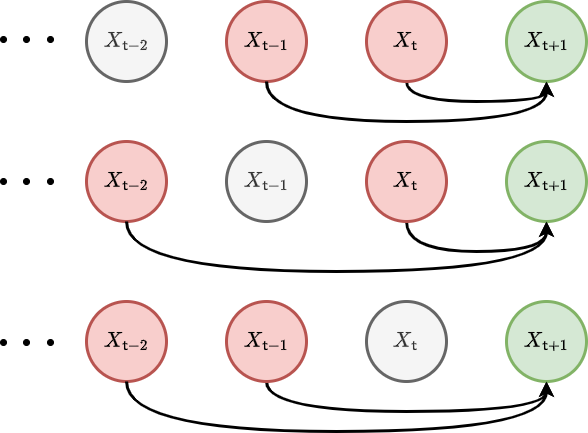
\includegraphics[width=8cm]{images/chapter-2-second-temporal-correlation.drawio.png}
\caption{A graph representation of the correlations in Eq.~(\ref{eq:second-order-correl}).}
\label{fig:second-temporal-correlation}
\end{figure} 

Given that the mean-field approach isn't always going to be viable as an inference method, we should also consider other ways to describe the shape and time evolution characteristics of $P_{{\sf t}+1}(X\vert z)$. For continuous state spaces, it's possible to approximate this whole distribution with a logarithmic expansion like so
%%
\begin{align}
\ln P_{{\sf t}+1}(X\vert z) &\simeq \ln P_{{\sf t}+1}(X_*\vert z) + \frac{1}{2}\sum_{{\sf t}'=0}^{{\sf t}+1}\sum_{i=0}^{n}\sum_{j=0}^{n} (x-x_*)^i {\cal H}^{ij}_{({\sf t}+1){\sf t}'}(z) (x'-x'_*)^j \label{eq:second-order-log-expansion} \\
{\cal H}^{ij}_{({\sf t}+1){\sf t}'}(z) &= \frac{\partial}{\partial x^i}\frac{\partial}{\partial (x')^j}\ln P_{{\sf t}+1}(X\vert z) \bigg\vert_{X=X_*} \label{eq:second-order-log-expansion-kernel} \,,
\end{align}
%% 
where the values for $X_*$ (and its rows $x_*, x_*', \dots$) are defined by the vanishing of the first derivative, i.e., these are chosen such that
%%
\begin{align}
\frac{\partial}{\partial x^i}\ln P_{{\sf t}+1}(X\vert z) \bigg\vert_{X=X_*} &= 0 \,.
\end{align}
%%
This logarithmic expansion is one way to see how a Gaussian process regression is able to approximate $X_{{\sf t}}$ evolving in time for many different processes. By selecting the appropriate function for the kernel given by Eq.~(\ref{eq:second-order-log-expansion-kernel}), a Gaussian process regression can be fully specified.

If we keep the truncation up to second order in Eq.~(\ref{eq:second-order-log-expansion}), note that this expression implies a pairwise correlation structure of the form
%%
\begin{align}
P_{{\sf t}+1}(X\vert z) &\rightarrow \prod_{{\sf t}'=0}^{{\sf t}}P_{({\sf t}+1){\sf t}'}(x,x'\vert z) = \prod_{{\sf t}'=0}^{{\sf t}}P_{{\sf t}'}(x'\vert z)P_{({\sf t}+1){\sf t}'}(x\vert x', z) \,.
\end{align}
%%
Given this pairwise temporal correlation structure, Eq.~(\ref{eq:master-x-cont-latest-row-gen}) reduces to this simpler sum of integrals
%%
\begin{align}
P_{{\sf t}+1}(x\vert z) &= \frac{1}{{\sf t}}\sum_{{\sf t}'=0}^{{\sf t}}\int_{\omega_{{\sf t}'}}{\rm d}^nx' P_{{\sf t}'}(x'\vert z)P_{({\sf t}+1){\sf t}'}(x\vert x',z) \label{eq:second-order-correl} \,.
\end{align}
%%
We have illustrated these second-order correlations with a graph visualisation in Fig.~(\ref{fig:second-temporal-correlation}).

\begin{figure}[h]
\centering
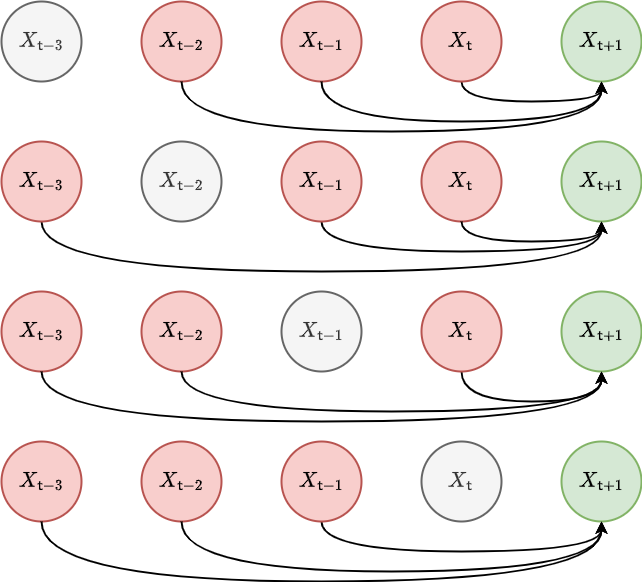
\includegraphics[width=10cm]{images/chapter-2-third-temporal-correlation.drawio.png}
\caption{A graph representation of the correlations in Eq.~(\ref{eq:third-order-correl}).}
\label{fig:third-temporal-correlation}
\end{figure}

In a similar fashion, we can increase the expansion order of Eq.~(\ref{eq:second-order-log-expansion}) to include third-order correlations such that 
%%
\begin{align}
P_{{\sf t}+1}(X\vert z) &\rightarrow \prod_{{\sf t}'=0}^{{\sf t}}\prod_{{\sf t}''=0}^{{\sf t}'-1} P_{{\sf t}'{\sf t}''}(x',x''\vert z)P_{({\sf t}+1){\sf t}'{\sf t}''}(x\vert x',x'',z) \,,
\end{align}
%%
and, in this instance, one can show that Eq.~(\ref{eq:master-x-cont-latest-row-gen}) reduces to
%%
\begin{align}
P_{{\sf t}+1}(x\vert z) &= \frac{1}{{\sf t}}\sum_{{\sf t}'=0}^{{\sf t}}\frac{1}{{\sf t}'-1}\sum_{{\sf t}''=0}^{{\sf t}'-1}\int_{\omega_{{\sf t}'}}{\rm d}^nx'\int_{\omega_{{\sf t}''}}{\rm d}^nx'' P_{{\sf t}'{\sf t}''}(x',x''\vert z)P_{({\sf t}+1){\sf t}'{\sf t}''}(x\vert x',x'',z) \label{eq:third-order-correl} \,.
\end{align}
%%
We have also illustrated these third-order correlations with another graph visualisation in Fig.~(\ref{fig:third-temporal-correlation}). Using $P_{{\sf t}'{\sf t}''}(x',x''\vert z) = P_{{\sf t}''}(x''\vert z) P_{{\sf t}'{\sf t}''}(x'\vert x'', z)$ one can also show that this integral is a marginalisation of this expression
%%
\begin{align}
P_{({\sf t}+1){\sf t}''}(x\vert x'', z) &= \frac{1}{{\sf t}}\sum_{{\sf t}'=0}^{{\sf t}}\int_{\omega_{{\sf t}'}}{\rm d}^nx'P_{{\sf t}'{\sf t}''}(x'\vert x'',z)P_{({\sf t}+1){\sf t}'{\sf t}''}(x\vert x',x'',z) \,,
\end{align}
%%
which describes the time evolution of the conditional probabilities. Note how this implies that the Gaussian process kernel itself can be evolved through time to replicate these higher-order temporal correlations for a regression problem, if desired.

Another probabilistic learning algorithm that we can consider is what we shall call `empirical probabilistic reweighting'. There is another expression for the mean of the distribution, that we can derive under certain conditions, which will be valuable to motivating this algorithm. If the probability distribution over each row of the state history matrix is \emph{stationary} --- meaning that $P_{{\sf t}+1}(x\vert z)=P_{{\sf t}'}(x\vert z)$ --- it's possible to go one step further than Eq.~(\ref{eq:mean-field-master}) and assert that
%%
\begin{align}
M_{{\sf t}+1}(z) &= \int_{\omega_{{\sf t}+1}}{\rm d}^nx \,x\,P_{{\sf t}+1}(x\vert z) = \frac{1}{{\sf t}}\sum_{{\sf t}'=0}^{{\sf t}}\int_{\omega_{{\sf t}'}}{\rm d}^nx' \,x'\, P_{{\sf t}'}(x'\vert z) \int_{\omega_{{\sf t}+1}}{\rm d}^nx\, P_{({\sf t}+1){\sf t}'}(x\vert x',z) \label{eq:stationary-mean-estimator}\,.
\end{align}
%%

To see that Eq.~(\ref{eq:stationary-mean-estimator}) is true, first note that a joint distribution over both $x$ and $x'$ can be derived like this $P_{({\sf t}+1){\sf t}'}(x,x'\vert z)=P_{({\sf t}+1){\sf t}'}(x\vert x',z)P_{{\sf t}'}(x'\vert z)$. Secondly, note that this joint distribution will always allow variable swaps trivially like this $P_{({\sf t}+1){\sf t}'}(x,x'\vert z)=P_{{\sf t}'({\sf t}+1)}(x',x\vert z)$. Then, lastly, note that stationarity of $P_{{\sf t}+1}(x\vert z)=P_{{\sf t}'}(x\vert z)$ means 
%%
\begin{align}
\frac{1}{{\sf t}}\sum_{{\sf t}'=0}^{{\sf t}}\int_{\omega_{{\sf t}+1}} {\rm d}^nx\int_{\omega_{{\sf t}'}} {\rm d}^nx' \,x\, P_{({\sf t}+1){\sf t}'}(x,x'\vert z)&=\frac{1}{{\sf t}}\sum_{{\sf t}'=0}^{{\sf t}}\int_{\omega_{{\sf t}'}} {\rm d}^nx\int_{\omega_{{\sf t}+1}} {\rm d}^nx' \,x\, P_{{\sf t}'({\sf t}+1)}(x,x'\vert z)\nonumber \\
&=\frac{1}{{\sf t}}\sum_{{\sf t}'=0}^{{\sf t}}\int_{\omega_{{\sf t}'}} {\rm d}^nx'\int_{\omega_{{\sf t}+1}} {\rm d}^nx \,x'\, P_{({\sf t}+1){\sf t}'}(x,x'\vert z) \nonumber \\
&=\frac{1}{{\sf t}}\sum_{{\sf t}'=0}^{{\sf t}}\int_{\omega_{{\sf t}'}}{\rm d}^nx' \,x'\, P_{{\sf t}'}(x'\vert z) \int_{\omega_{{\sf t}+1}}{\rm d}^nx\, P_{({\sf t}+1){\sf t}'}(x\vert x',z)\nonumber \,,
\end{align}
%%
where we've used the trivial variable swap and integration variable relabelling to arrive at the second equality in the expressions above. 

The standard covariance matrix elements can also be computed in a similar fashion
%%
\begin{align}
C^{ij}_{{\sf t}+1}(z) &= \int_{\omega_{{\sf t}+1}}{\rm d}^nx \,[x-M_{{\sf t}+1}(z)
]^i[x-M_{{\sf t}+1}(z)]^jP_{{\sf t}+1}(x\vert z) \nonumber \\
&= \frac{1}{{\sf t}}\sum_{{\sf t}'=0}^{{\sf t}}\int_{\omega_{{\sf t}'}}{\rm d}^nx' \, [x'-M_{{\sf t}+1}(z)]^i[x'-M_{{\sf t}+1}(z)]^j \,P_{{\sf t}'}(x'\vert z) \int_{\omega_{{\sf t}+1}}{\rm d}^nx \, P_{({\sf t}+1){\sf t}'}(x\vert x',z) \label{eq:stationary-covariance-estimator}\,.
\end{align}
%%
While they look quite abstract, Eqs.~(\ref{eq:stationary-mean-estimator}) and~(\ref{eq:stationary-covariance-estimator}) express the core idea behind how the probabilistic reweighting will function. By assuming a stationary distribution, we gain the ability to directly estimate the statistics of the probability distribution of the next sample from the stochastic process $P_{{\sf t}+1}(x\vert z)$ from past samples it may have in empirical data; which are represented here by $P_{{\sf t}'}(x'\vert z)$.

Probabilistic reweighting depends on the stationarity of $P_{{\sf t}+1}(x\vert z)=P_{{\sf t}'}(x\vert z)$ such that, e.g., Eq.~(\ref{eq:stationary-mean-estimator}) is applicable. The core idea behind it is to represent the past distribution of state values $P_{{\sf t}'}(x'\vert z)$ with the samples from a real time series dataset. If the user then specifies a good model for the relationships in this data by providing a weighting function which returns the conditional probability mass
%%
\begin{align}
{\sf w}_{{\sf t}'}(y,z) = \int_{\omega_{{\sf t}+1}} {\rm d}^nx \, P_{({\sf t}+1){\sf t}'}(x\vert x'{=}y,z) \,,  
\end{align}
%%
we can apply this as a \emph{reweighting} of the historical time series samples to estimate any statistics of interest. Taking Eqs.~(\ref{eq:stationary-mean-estimator}) and~(\ref{eq:stationary-covariance-estimator}) as the examples; we are essentially approximating these integrals through weighted sample estimations like this
%%
\begin{align}
M_{{\sf t}+1}(z) &\simeq \frac{1}{{\sf t}}\sum^{{\sf t}}_{{\sf t}'=0}Y_{{\sf t}'} {\sf w}_{{\sf t}'}(Y_{{\sf t}'},z) \label{eq:mean-reweighting} \\
C^{ij}_{{\sf t}+1}(z) &\simeq \frac{1}{{\sf t}}\sum^{{\sf t}}_{{\sf t}'=0}[Y_{{\sf t}'}-M_{{\sf t}+1}(z)]^i[Y_{{\sf t}'}-M_{{\sf t}+1}(z)]^j \, {\sf w}_{{\sf t}'}(Y_{{\sf t}'},z) \label{eq:covariance-reweighting} \,,
\end{align}
%%
where we have defined the data matrix $Y$ with rows $Y_{{\sf t}+1}, Y_{{\sf t}}, \dots$, each of which representing specific observations of the rows in $X$ at each point in time from a real dataset.

The goal of a learning algorithm for probabilistic reweighting would be to learn the optimal reweighting function ${\sf w}_{{\sf t}'}(Y_{{\sf t}'},z)$ with respect to $z$, i.e., the ones which most accurately represent a provided dataset. But before we think about the various kinds of conditional probability we could use, we need to think about how to connect the post-reweighting statistics to the data by defining an objective function. 

If the mean is a sufficient statistic for the distribution which describes the data, a choice of, e.g., Exponential, Poisson or Binomial distribution could be used where the mean is estimated directly from the time series using Eq.~(\ref{eq:stationary-mean-estimator}), given a conditional probability $P_{({\sf t}+1){\sf t}'}(x\vert x',z)$. Extending this idea further to include distributions which also require a variance to be known, e.g., the Normal, Gamma or Negative Binomial distributions could be used where the variance (and/or covariance) could be estimated using Eq.~(\ref{eq:stationary-covariance-estimator}). These are just a few simple examples of distributions that can link the estimated statistics from Eqs.~(\ref{eq:stationary-mean-estimator}) and~(\ref{eq:stationary-covariance-estimator}) to a time series dataset. However, the algorithmic framework is very general to whatever choice of `data linking' distribution that a researcher might need.

We should probably make what we've just said a little more mathematically concrete. We can define $P_{{\sf t}+1}[y;M_{{\sf t}+1}(z),C_{{\sf t}+1}(z),\dots ]$ as representing the likelihood of $y = Y_{{\sf t}+1}$ given the estimated statistics from Eqs.~(\ref{eq:stationary-mean-estimator}) and~(\ref{eq:stationary-covariance-estimator}) (and maybe higher-orders). Note that in order to do this, we need to identify the $x'$ and ${\sf t}'$ values that are used to estimate, e.g., $M_{{\sf t}+1}(z)$ with the past data values which are observed in the dataset time series itself. Now that we have this likelihood, we can immediately evaluate an objective function (a cumulative log-likelihood) that we might seek to optimise over for a given dataset 
%%
\begin{align}
\ln {\cal L}_{{\sf t}+1}(Y\vert z) &= \sum_{{\sf t}'=0}^{{\sf t}+1} \ln P_{{\sf t}'}[y;M_{{\sf t}'}(z),C_{{\sf t}'}(z),\dots ] \,, \label{eq:log-likelihood-reweighting}
\end{align}
%%
where the summation continues until all of the past measurements $Y_{{\sf t}+1}, Y_{{\sf t}}, \dots$ which exist as rows in the data matrix $Y$ have been taken into account. The code to compute this objective function follows the schematic we have provided in Fig.~\ref{fig:prob-reweighting-code}.

\begin{figure}[h]
\centering
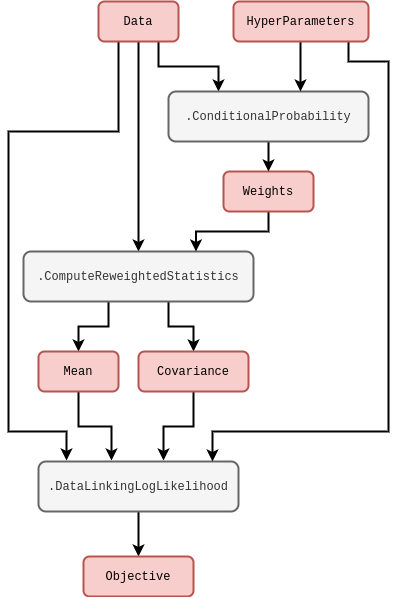
\includegraphics[width=8cm]{images/chapter-2-prob-reweighting-code.drawio.png}
\caption{Code schematic of the probability reweighting objective computation.}
\label{fig:prob-reweighting-code}
\end{figure} 

In order to specify what $P_{({\sf t}+1){\sf t}'}(x\vert x',z)$ is, it's quite natural to define a set of hyperparameters for the elements of $z$. To get a sense of how the data-linking function relates to these hyperparameters, it's instructive to consider an example. One generally-applicable option for the conditional probability could be a purely time-dependent kernel
%%
\begin{align}
P_{({\sf t}+1){\sf t}'}(x\vert x',z) &\propto {\cal K}(z, {\sf t}+1,{\sf t}')  \label{eq:time-dependent-kernel} \,, 
\end{align}
%%
and the data-linking distribution, e.g., could be a Gaussian
%%
\begin{align}
P_{{\sf t}+1}[y;M_{{\sf t}+1}(z),C_{{\sf t}+1}(z),\dots ] = {\sf MultivariateNormalPDF}[y;M_{{\sf t}+1}(z),C_{{\sf t}+1}(z)] \label{eq:gaussian-data-prob}\,.
\end{align}
%%
It's worth pointing out that other machine learning frameworks could easily be used to model these conditional probabilities. For example, neural networks could be used to infer the optimal reweighting scheme and this would still allow us to use the data-linking distribution.\footnote{One can think of using this neural network-based reweighting scheme as similar to constructing a normalising flow model~\cite{kobyzev2020normalizing} with an autoregressive layer. Invertibility and further network structural constraints mean that these are not exactly equivalent, however.} It would still be desirable to keep the data-linking distribution as it can usually be sampled from very easily --- something that can be quite difficult to achieve with a purely machine learning-based representation of the distribution. Sampling itself could even be made more flexible by leveraging a Variational Autoencoder (VAE)~\cite{pinheiro2021variational}; these use neural networks not just on the compression (or `encode') step to estimate the statistics but also use them as a layer between the sample from the data distribution model and the output (the `decode' step).

In the case of Eqs.~(\ref{eq:time-dependent-kernel}) and~(\ref{eq:gaussian-data-prob}) above, the hyperparameters that would be optimised could relate to the kernel in a wide variety of ways. Optimising them would make our optimised reweighting similar to (but very much \emph{not} the same as) evaluating maximum a posteriori (MAP) of a Gaussian process regression. In a Gaussian process regression, one is concerned with inferring the the whole of $X_{{\sf t}}$ as a function of time using the pairwise correlations implied by Eq.~(\ref{eq:second-order-log-expansion}). Based on this expression, the cumulative log-likelihood for a Gaussian process can be calculated as follows
%%
\begin{align}
\ln {\cal L}_{{\sf t}+1}(Y\vert z) &= -\frac{1}{2}\sum_{{\sf t}'=0}^{{\sf t}+1}\sum_{{\sf t}''=0}^{{\sf t}'} \bigg[ n\ln (2\pi ) + \ln \big\vert {\cal H}_{{\sf t}'{\sf t}''}(z)\big\vert + \sum_{i=0}^{n}\sum_{j=0}^{n} Y^i_{{\sf t}'} {\cal H}^{ij}_{{\sf t}'{\sf t}''}(z) Y^j_{{\sf t}''} \bigg] \,. \label{eq:log-likelihood-gaussian-proc}    
\end{align}
%%

As we did for the reweighting algorithm, in Fig.~\ref{fig:gaussian-process-code} we have illustrated a schematic of the basic code needed to compute the objective function of a learning algorithm based on Eq.~(\ref{eq:log-likelihood-gaussian-proc}). Note that, in the expression above, we have assumed that the data has already been shifted such that its values are positioned around the distribution peak. Knowing where this peak will be a priori is not possible. However, for Gaussian data, an unbiased estimator for this peak will be the sample mean and so we have included an initial data standardisation in the steps outlined by Fig.~\ref{fig:gaussian-process-code}.

\begin{figure}[h]
\centering
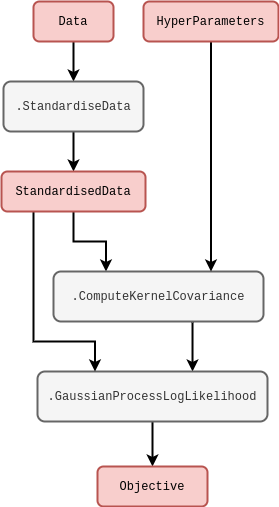
\includegraphics[width=6cm]{images/chapter-2-gaussian-process-code.drawio.png}
\caption{Code schematic of the Gaussian process objective computation.}
\label{fig:gaussian-process-code}
\end{figure}

The optimisation approach that we choose to use for obtaining the best hyperparameters in the conditional probability of Eq.~(\ref{eq:log-likelihood-reweighting}) will depend on a few factors. For example, if the number of hyperparameters is relatively low, but their gradients are difficult to calculate exactly; then a gradient-free optimiser (such as the Nelder-Mead~\cite{nelder1965simplex} method or something like a particle swarm~\cite{kennedy1995particle, shi1998modified}) would likely be the most effective choice. On the other hand, when the number of hyperparameters ends up being relatively large, it's usually quite desriable to utilise the gradients in algorithms like vanilla Stochastic Gradient Descent~\cite{robbins1951stochastic} (SGD) or Adam~\cite{kingma2014adam}.

If the gradients of Eq.~(\ref{eq:log-likelihood-reweighting}) are needed, we can always factorise each derivative with respect to hyperparameter $z^i$ in the following way through the chain rule
%%
\begin{align}
\frac{\partial}{\partial z^i}\ln {\cal L}_{{\sf t}+1}(Y \vert z) &= \sum_{{\sf t}'=0}^{{\sf t}+1}\frac{\partial M_{{\sf t}'}}{\partial z^i}\frac{\partial}{\partial M_{{\sf t}'}}\ln P_{{\sf t}'}[y;M_{{\sf t}'}(z),C_{{\sf t}'}(z),\dots ] \nonumber \\
&\qquad + \sum_{{\sf t}'=0}^{{\sf t}+1}\frac{\partial C_{{\sf t}'}}{\partial z^i}\frac{\partial }{\partial C_{{\sf t}'}}\ln P_{{\sf t}'}[y;M_{{\sf t}'}(z),C_{{\sf t}'}(z),\dots ] \,. \label{eq:log-likelihood-reweighting-grad}
\end{align}
%%
By factoring derivatives in this manner, the computation can be separated into two parts: the derivatives with respect to $M_{{\sf t}'}$ and $C_{{\sf t}'}$, which are typically quite straightforward; and the derivatives with respect to $z$ elements, which typically need a more involved calculation depending on the model. Incidentally, this separation also neatly lends itself to abstracting gradient calculations as having a simpler, general purpose component that can be built directly into a library of data models and a more complex, model-specific component that the user must specify.

The same logic should apply to a learning algorithm which optimises $z$ to obtain the MAP for a Gaussian process. If the gradients of Eq.~(\ref{eq:log-likelihood-gaussian-proc}) are required, the user would have to specify derivatives of the kernel matrix (and its determinant) with respect to each hyperparameter $z^k$ in order to calculate
%%
\begin{align}
\frac{\partial}{\partial z^k}\ln {\cal L}_{{\sf t}+1}(Y \vert z) &= -\frac{1}{2}\sum_{{\sf t}'=0}^{{\sf t}+1}\sum_{{\sf t}''=0}^{{\sf t}'} \bigg[ \frac{\partial}{\partial z^k}\ln \big\vert {\cal H}_{{\sf t}'{\sf t}''}(z)\big\vert + \sum_{i=0}^{n}\sum_{j=0}^{n} Y^i_{{\sf t}'} \frac{\partial}{\partial z^k}{\cal H}^{ij}_{{\sf t}'{\sf t}''}(z)Y^j_{{\sf t}''} \bigg] \,. \label{eq:log-likelihood-gaussian-proc-grad}
\end{align}
%%

\section{\sffamily Online learning with any algorithm}

We have discussed the importance of probabilistic learning in the context of environments where only partial state observability is possible and, in the previous chapter, we motivated the use of some specific probabilistic learning methods. However, we haven't yet discussed how we might implement a learning algorithm in practice. In particular, before covering the various aspects of software design, it's important to consider how we want to structure learning by optimisation of an objective with respect to a stream of time series data.

One of the issues that can arise when learning streams of data is `concept drift'. In our context, this would be when the optimal value for $z$ does not match the optimal value at some later point in time. In order to mitigate this, our learning algorithms should be able to track an up-to-date optimal value for $z$ as data is continually passed into them. Iteratively updating the optimal parameters as new data is ingested into the objective function is typically called `online learning'~\cite{hazan2016introduction,sutton2018reinforcement}, in contrast to `offline learning' which would correspond to learning an optimal $z$ only once with the entire dataset provided upfront.

The reader may recall that this book is about building more realistic environments for machine learning systems. An important part of learning from environments in a robust manner is ensuring \emph{adaptability to new data}. In addition to this, stochastic processes are inherently sequential. Many types of system evolve not just their states, but also dynamical description, over time. Online learning is the natural framework to use in this context.

Let's return to the models we discussed in the previous chapter which optimise the cumulative log-likelihood of the data matrix $Y$ with respect to $z$ at a particular point in time, i.e., which optimise $\ln {\cal L}_{{\sf t}+1}(Y\vert z)$ with respect to $z$ at time ${\sf t}+1$. The simplest (and most generally applicable) way to implement an online learning approach with any machine learning model is to rerun the whole optimisation algorithm for $z$ after each new datapoint $y$ has been received. Each time the optimisation is rerun, it will be using the entire batch of training data --- here represented by the data matrix $Y$. This kind of `batch' online learning will work for most of the standard machine learning algorithms, but the re-training process can take a long time to run in each instance. 

One way to speed things up is to assume that the optimal value for $z$ which was obtained from the previous data iterations is close to the one we will find in the most recent iteration. Hence, by inserting this previous value into the next run of the optimisation procedure as an initial guess, the algorithm will typically converge much more quickly to the optimum. This is more of a practical insight, but are there any quantitative methods which can reduce the amount of computation required to update $z$ when the latest datapoint in the series has been received?

This is where `pure' online learning comes in. When gradients of the log-likelihood are available, we can make things much more efficient. Consider ${\cal L}_{{\sf t}+1}(y\vert z)$ as the log-likelihood term for datapoint $y$ such that the cumulative log-likelihood of the data matrix $Y$ can be written as the following summation of terms
%%
\begin{align}
\ln {\cal L}_{{\sf t}+1}(Y\vert z) = \sum^{{\sf t}+1}_{{\sf t}'=0}\ln {\cal L}_{{\sf t}'}(y\vert z)\,.
\end{align}
%%
If we now denote the $z$ which we have learned from the data up to timestep ${\sf t}$ as $z_*({\sf t})$, we may write the following expression which uses the gradient of the log-likelihood to learn from each new datapoint arrival
%%
\begin{align}
z^i_*({\sf t}+1) &= z^i_*({\sf t}) - \alpha ({\sf t}+1,\dots ) \frac{\partial}{\partial z^i} \ln {\cal L}_{{\sf t}+1}(y\vert z) \label{eq:sgd-online} \,,
\end{align}
%%
which is based on a stochastic gradient descent (SGD) algorithm approach. In contrast to the more standard offline SGD approach --- which would be applied to mini-batches of the data --- this update is applied to $z_*$ using the log-likelihood at each point in time in sequence.

In Eq.~(\ref{eq:sgd-online}) the $\alpha ({\sf t}+1,\dots )$ function, or `learning rate' function, returns a value which controls the step size towards the optimal value. As indicated by the arguments to this function, the learning rate can be time-dependent, which allows the user to set a schedule of steps which help convergence in certain problems. Other inputs can depend on the specific flavour of stochastic gradient descent algorithm that is being run. For example, an Adam optimiser~\cite{kingma2014adam} makes use of the statistics computed from the history of gradient values obtained as the algorithm progresses.

\textcolor{red}{Still need to discuss:
\begin{itemize}
\item{batch learning algorithms --- more like Gaussian processes}
\item{`pure' online learning algorithms --- more like empirical probabilistic reweighting}
\end{itemize}}

\textcolor{red}{Got to here in rewrite...}

Note that other excellent online machine learning frameworks are available --- see, e.g., River~\cite{river} and Vowpal Wabbit~\cite{vowpalwabbit}. The motivation for designing our own probabilistic online learning software is to ensure maximal integration with the stochadex simulation engine. We'll aim to achieve this by designing the code to use the same data structures and and concepts as we used when building the stochadex, where possible. In the next section on software design, we will show how this can be done while still maintaining extensibility and interoperability with other machine learning libraries and APIs. So let's get on with it!

\section{\sffamily Simulation inference formalism}

In Bayesian inference, one applies Bayes' rule to the problem of statistically inferring a model from some dataset. This typically involves the following formula for a posterior distribution
%%
\begin{align}
{\cal P}_{{\sf t}+1}(z \vert Y) \propto {\cal L}_{{\sf t}+1}(Y\vert z){\cal P} (z) \label{eq:bayes-rule} \,.
\end{align}
%%
In the formula above, one relates the prior probability distribution over a parameter set ${\cal P} (z)$ and the likelihood ${\cal L}_{{\sf t}+1}(Y\vert z)$  of some data matrix $Y$ up to timestep ${\sf t}+1$ given the parameters $z$ of a model to the posterior probability distribution of parameters given the data ${\cal P}_{{\sf t}+1}(z \vert Y)$ up to some proportionality constant. All this may sound a bit technical in statistical language, so it can also be helpful to summarise what the formula above states verbally as follows: the initial (prior) state of knowledge about the parameters $z$ we want to learn can be updated by some likelihood function of the data to give a new state of knowledge about the values for $z$ (the `posterior' probability). 

From the point of view of statistical inference, if we seek to maximise ${\cal P}_{{\sf t}+1}(z \vert Y)$ --- or its logarithm --- in Eq.~(\ref{eq:bayes-rule}) with respect to $z$, we will obtain what is known as a maximum posteriori (MAP) estimate of the parameters. In fact, we have already encountered this metholodology in the previous chapter when discussing the algorithm which obtains the best fit parameters for the empirical probability reweighting. In this case; while it appears that we optimised the log-likelihood directly as our objective function, one can easily show that this is also technically equivalent obtaining a MAP estimate where one chooses a specfic prior ${\cal P} (z) \propto 1$ (typically known as a `flat prior').

How might we calulate the posterior in practice with some arbitrary stochastic process model that has been defined in the stochadex? In order to make the comparison to a real dataset, any stochadex model of interest will always need to be able to generate observations which can be directly compared to the data. To formalise this a little; a stochadex model could be represented as a map from $z$ to a set of stochastic measurements ${\sf Y}_{{\sf t}+1}(z), {\sf Y}_{{\sf t}}(z), \dots$ that are directly comparable to the rows in the real data matrix $Y$. The values in $Y$ may only represent a noisy or partial measurement of the latent states of the simulation $X$, so a more complete picture can be provided by the following probabilistic relation
%%
\begin{align}
P_{{\sf t}+1}({\sf y} \vert z) = \int_{\omega_{{\sf t}+1}}{\rm d}^nx\, P_{{\sf t}+1}({\sf y} \vert x)P_{{\sf t}+1}(x \vert z) \,, \label{eq:simulation-measurement}
\end{align}
%%
where, in practical terms, the measurement probability $P_{{\sf t}+1}({\sf y} \vert x)$ of ${\sf Y}_{{\sf t}+1}={\sf y}$ given $X_{{\sf t}+1}=x$ can be represented by sampling from another stochastic process which takes the state of the stochadex simulation as input. Given that we have this capability to compare like-for-like between the data and the simulation; the next problem is to figure out how this comparison between two sequences of vectors can be done in a way which ensures the the statistics of the posterior are ultimately respected. 

For an arbitrary simulation model which is defined by the stochadex, the likelihood in Eq.~(\ref{eq:bayes-rule}) is typically not describable as a simple function or distribution. While we could train the probability reweighting we derived in the previous chapter to match the simulation; to do this well would require having an exact formula for the conditional probability, and this is not always easy to derive in the general case. Instead, there is a class of Bayesian inference methods which we shall lean on to help us compute the posterior distribution (and hence the MAP), which are known as `Likelihood-Free' methods~\cite{sisson2018handbook,price2018bayesian,wood2010statistical,drovandi2022comparison}.

`Likelihood-Free' methods work by separating out the components of the posterior which relate to the closeness of rows in ${\sf Y}$ to the rows in $Y$ from the components which relate the states $X$ and parameters $z$ of the simulation stochastically to ${\sf Y}$. To achieve this separation, we can make use of chaining conditional probability like this
%%
\begin{align}
{\cal P}_{{\sf t}+1}(X,z\vert Y)=\int_{\Upsilon_{{\sf t}+1}} {\rm d}{\sf Y} \, {\cal P}_{{\sf t}+1}({\sf Y}\vert Y) P_{{\sf t}+1}(X,z \vert {\sf Y}) \label{eq:likelihood-free-posterior} \,,
\end{align}
%%
where $\Upsilon_{{\sf t}+1}$ here corresponds to the domain of the simulated measurements matrix ${\sf Y}$ at time ${\sf t}+1$.

As we demonstrated in the previous chapter, it's possible for us to also optimise a probability distribution ${\cal P}_{{\sf t}'}({\sf y}\vert Y) = P_{{\sf t}'}({\sf y};{\cal M}_{{\sf t}'},{\cal C}_{{\sf t}'},\dots )$ for each step in time to match the statistics of the measurements in $Y$ as well as possible, given some statistics ${\cal M}_{{\sf t}'}={\cal M}_{{\sf t}'}(Y)$ and ${\cal C}_{{\sf t}'}={\cal C}_{{\sf t}'}(Y)$. Assuming the independence of samples (rows) in $Y$, this distribution can be used to construct the distribution over all of $Y$ through the following product
%%
\begin{align}
{\cal P}_{{\sf t}+1}({\sf Y}\vert Y) = \prod_{{\sf t}'=0}^{{\sf t}+1}P_{{\sf t}'}({\sf y};{\cal M}_{{\sf t}'},{\cal C}_{{\sf t}'},\dots ) \,.
\end{align}
%%
We do not necessarily need to obtain these statistics from the probability reweighting method, but could instead try to fit them via some other objective function. Either way, this represents a lossy \emph{compression} of the data we want to fit the simulation to, and so the best possible fit is desirable; regardless of overfitting. This choice to summarise the data with statistics means we are using what is known as a Bayesian Synthetic Likelihood (BSL) method~\cite{price2018bayesian,wood2010statistical} instead of another class of methods which approximate an objective function directly using a proximity kernel --- known as Approximate Bayesian Computation (ABC) methods~\cite{sisson2018handbook}.

Let's consider a few concrete examples of $P_{{\sf t}'}({\sf y};{\cal M}_{{\sf t}'},{\cal C}_{{\sf t}'}, \dots )$. If the data measurements were well-described by a multivariate normal distribution, then
%%
\begin{align}
P_{{\sf t}'}({\sf y};{\cal M}_{{\sf t}'},{\cal C}_{{\sf t}'}, \dots ) = {\sf MultivariateNormalPDF}({\sf y};{\cal M}_{{\sf t}'},{\cal C}_{{\sf t}'})\,,
\end{align}
%%
Similarly, if the data measurements were instead better described by a Poisson distribution, we might disregard the need for a covariance matrix statistic ${\cal C}_{{\sf t}'}$ and instead use
%%
\begin{align}
P_{{\sf t}'}({\sf y};{\cal M}_{{\sf t}'},{\cal C}_{{\sf t}'}, \dots ) = {\sf PoissonPMF}({\sf y};{\cal M}_{{\sf t}'})\,.
\end{align}
%%
The more statistically-inclined readers may notice that the probability mass function here would require the integrals in Eq.~(\ref{eq:likelihood-free-posterior}) to be replaced with summations over the relevant domains.

Eq.~(\ref{eq:likelihood-free-posterior}) demonstrates how one can construct a statistically meaningful way to compare the sequence of real data measurements $Y_{{\sf t}+1}, Y_{{\sf t}}, \dots$ to their modelled equivalents ${\sf Y}_{{\sf t}+1}(z), {\sf Y}_{{\sf t}}(z), \dots$. But we still haven't shown how to compute $P_{{\sf t}+1}(X,z\vert {\sf Y})$ for a given simulation, and this can be the most challenging part. To begin with, we can reapply Bayes' rule and the chaining of conditional probability to find 
%%
\begin{align}
P_{{\sf t}+1}(x,z\vert {\sf Y}) \propto P_{{\sf t}+1}({\sf y}\vert z)P_{{\sf t}}(z\vert {\sf Y}') = P_{{\sf t}+1}({\sf y}\vert x)P_{{\sf t}+1}(x\vert z)P_{{\sf t}}(z\vert {\sf Y}') \,,
\end{align}
%%
where here $P_{{\sf t}}(z\vert {\sf Y}')$ is the probability of ${\sf Y}_{{\sf t}}={\sf Y}'$.

The relationship between $P_{{\sf t}+1}(X\vert z)$ and previous timesteps can be directly inferred from the probabilistic iteration formula that we introduced in the previous chapter. So we can map probabilities of $X_{0:{\sf t}+1} = X$ throughout time and learned information about the state of the system can be applied from previous values, given $z$. But is there a similar relationship we might consider for $P_{{\sf t}+1}(z\vert {\sf Y})$? Yes there is! The marginalisation
%%
\begin{align} 
P_{{\sf t}+1}(z\vert {\sf Y}) &\propto \bigg[ \int_{\Omega_{{\sf t}+1}} {\rm d}^nx \,P_{{\sf t}+1}({\sf y}\vert x) P_{{\sf t}+1}(x\vert z) \bigg] P_{{\sf t}}(z\vert {\sf Y}') \label{eq:z-update}\,,
\end{align}
%%
shows how the $z$ updates can occur in an iterative fashion. The reader may also recognize the factor above in brackets as Eq.~(\ref{eq:simulation-measurement}). To complete the picture, one can combine the $X$ and $z$ updates into a joint distribution update which takes the following form 
%%
\begin{align} 
P_{{\sf t}+1}(X,z\vert {\sf Y}) &\propto P_{{\sf t}+1}({\sf y}\vert x) P_{({\sf t}+1){\sf t}}(x\vert X', z) P_{{\sf t}}(X',z\vert {\sf Y}') \label{eq:x-z-update}\,.
\end{align}
%%
We can also marginalise this distribution over the past state history rows to get a distribution over the latest state row $X_{{\sf t}+1}=x$ like this 
%%
\begin{align}
P_{{\sf t}+1}(x,z\vert {\sf Y}) &= \int_{\Omega_{{\sf t}}} {\rm d}X'P_{{\sf t}+1}(X,z\vert {\sf Y}) \propto P_{{\sf t}+1}({\sf y}\vert x) \int_{\Omega_{{\sf t}}} {\rm d}X' P_{({\sf t}+1){\sf t}}(x\vert X', z) P_{{\sf t}}(X',z\vert {\sf Y}') \label{eq:x-z-update-latest-row} \,.
\end{align}
%%

In the next section, we're going to discuss how to translate all of this probabilistic language into some MAP inference algorithms. Before we do this, however, it will be instructive (particularly for `online' learning algorithms) to consider what happens if the model changes over time and $z$ needs to change in order to better represent the real data. In such situations, we propose to apply the same formula as Eq.~(\ref{eq:x-z-update-latest-row}) but instead replace the distribution over $(X',z)$ on the right hand side with its `past discounted' version\footnote{In the continuous-time version, this past-discounting factor can depend on the stepsize such that we replace
$$
\beta^{{\sf t}-{\sf t}'} \longrightarrow \frac{1}{\beta [\delta t({\sf t})]}\prod_{{\sf t}''={\sf t}'}^{{\sf t}} \beta [\delta t({\sf t}'')] \,.
$$}
\textcolor{red}{Formula below is wrong --- reformulate in terms of a $\beta^{{\sf t}-{\sf t}'}$ Bayesian evidence weighting factor for each past timestep and the result will be a $\prod$ expression here not a $\sum$...} 
%%
\begin{align}
\int_{\Omega_{{\sf t}}}{\rm d}X' P_{{\sf t}}(X',z\vert {\sf Y}') \,\, \longrightarrow \,\, \frac{1}{{\sf t}}\sum_{{\sf t}'=0}^{{\sf t}}\int_{\omega_{{\sf t}'}}{\rm d}^nx' \beta^{{\sf t}-{\sf t}'} P_{{\sf t}'}(x',z\vert {\sf Y}') \,,
\end{align}
%%
where $0 < \beta < 1$ and we recall the notation which considers distributions over the individual rows $x'$ within the matrix $X'$ in this new version. This time-dependent discount factor could be used to reduce the dependence of the update on data which is much further in the past, and hence will ultimately lead to a more responsive algorithm. This responsiveness would have to be balanced with the tradeoffs associated with discounting potentially valuable data that may offer greater long-term stability. Readers who are familiar with reinforcement learning may be starting to feel in familiar territory here --- they will have to wait for the latter parts of the book to see more on discounting though!

\section{\sffamily Online learning the MAP}

Eq.~(\ref{eq:x-z-update}) tells us how to probabilistically translate the current state of knowledge about $(x,z)$ forward through time in response to the arrival of new data. We also know how to connect the simulated measurements to the real data because Eq.~(\ref{eq:likelihood-free-posterior}) essentially gives us an objective function to maximise for each step in time. This is all great in theory; but in practice, this optimisation problem typically has several layers of difficulty to it. Since the model has been defined by its stochastically generated samples of measurements ${\sf Y}_{{\sf t}+1}(z), {\sf Y}_{{\sf t}}(z), \dots$, the objective function will manifestly be stochastic too. Another layer of difficulty is that gradients of the objective function are not immediately computable and so navigation around the optimisation domain could be difficult, especially in high-dimensional problems. Lastly, given that the simulation model in the stochadex needs to be running multiple times for each timestep, we need a way of mitigating computational expense. 

So how should we proceed? To solve this problem in the general case, Eqs.~(\ref{eq:likelihood-free-posterior}) and~(\ref{eq:x-z-update}) tell us we need to synthesize the following components into a single algorithm:
%%
\begin{enumerate}
\item{A process $P_{({\sf t}+1){\sf t}}(x\vert X', z)$ which iterates the state matrix of the simulation $X$ forward in time.}
\item{A process $P_{{\sf t}+1}({\sf y}\vert x)$ which generates a simulated measurement from the simulated state $x$.}
\item{A probability distribution $P_{{\sf t}'}({\sf y};{\cal M}_{{\sf t}'},{\cal C}_{{\sf t}'}, \dots )$ which represents the posterior distribution of the simulated measurement vector ${\sf y}$ given an optimised compression of the real data into summary statistics.}
\item{Some way of representing samples from the distribution $P_{{\sf t}+1}(X,z\vert {\sf Y})$ so that their distribution can be updated and will coverge towards the posterior over $(X,z)$.}
\end{enumerate}
%%

\textcolor{red}{Cite this nice paper which outlines all the recent kinds of simulation inference:~\cite{cranmer2020frontier}.}

\textcolor{red}{Keep the heuristic Bayes posterior estimator method as it is an example of recursive Bayes estimation - it can also be used to filter the ensemble at every step to make a particle filter~\cite{arulampalam2002tutorial}. Amortize this online learning process by training a neural net to produce the best estimates for the filter from the input real data!}

\textcolor{red}{
Before writing this up, should read this paper on efficient amortized inference using neural networks with \texttt{BayesFlow} here in particular:~\cite{radev2020bayesflow}. But also, should cite other works to make amortized inference more efficient by using neural networks to learn convenient functions of the Bayes factor in Evidence networks~\cite{jeffrey2023evidence}.
\begin{itemize}
\item{amortized online inference of the posterior update over just $z$ can be 
achieved by running lots of simulations and solving the inverse problem with the ${\sf y}$ outputs
i.e., neural network modelling of the update in Eq.~(\ref{eq:z-update})} 
\end{itemize}
}


\textcolor{red}{The algorithm is specifically: 
1. if this is a refit step, sample new values for $(X,z)$ for all members of the ensemble from the current $(X,z)$ distribution points and run the iterations for all of these ensemble members from the back of the window all the way up to the current point in time (hence the full matrix $X$ is sampled)
2. take all of the ensemble members a step forward in time
3. approximate the mode by computing the average values of $z$ within the $q$-th percentile of the sampled probability mass (where $q$ is set by the user and is ideally < 68\%) --- this idea comes from nested sampling
4. stream in the data for the next point in time and go to 1.}


As such an algorithm converges, we can recompute (and hence iteratively improve) the MAP estimate with respect to each iteration of the posterior.

Readers with some machine learning experience may be familiar with the classic exploration vs exploitation tradeoffs. It's clear that these tradeoffs will manifest in our case here when trying to strike a balance between iterating the posterior distribution and optimizing the current posterior with respect to $(X,z)$ to compute the MAP. 

Readers of the previous section may also have recognized that Eq.~(\ref{eq:x-z-update}) contains the same conditional probability $P_{({\sf t}+1){\sf t}}(x\vert X',z)$ as the reweighting algorithm. This structure enables us to reuse all of the exposition we provided for the probabilistic reweighting and highlights how the reweighting itself can be used in the algorithm to optimise the posterior.   

If we now synthesize both of these observations together, we can see how a stochastic variant of the well-known Expectation-Maximisation Algorithm~\cite{hartley1958maximum, dempster1977maximum, murphy2012machine} naturally emerges.

\section{\sffamily Software design}

Let's now take a step back from the specifics of the probabilistic reweighting algorithm to introduce our new sofware package for this part of the book: the `learnadex'. At its core, the learnadex algorithm adapts the stochadex iteration engine to iterate through streams of data in order to accumulate a global objective function value with respect to that data. The user may then choose which optimisation algorithm (or write their own) to use in order to leverage this objective for learning a better representation of the data. 

As we discussed at the end of the last section, the algorithms in the learnadex are all applied in an `online' fashion --- refitting for the optimal hyperparameters $z$ as new data is streamed into them. A challenging aspect of online learning is in managing the computational expense of recomputing the optimal value for $z$ after each new datapoint is sent. To help with this; the user may configure the algorithm recompute the optimum value after larger batches of data have been ingested. The last value of optimum $z$ will also frequently be close to the next optimum in the sequence, so using the former as the initial input into the optimisation routine for the latter is typically very valuable for aiding efficiency.

Reusing the \texttt{PartitionCoordinator} code of the stochadex to facilitate online learning makes neat use of software which has already been designed and tested in earlier chapters of this book. However, in order to fully achieve this, an additional configuration type is necessary; as we show in Fig.~\ref{fig:learnadex-data-types-design}. To start with, we separate out `learning' from the kind of optimiser in the overall config so as to enable multiple optimisation algorithms to be used for the same learning problem. The hyperparameters that define that optimisation problem domain can be determined by the user with an extension to the \texttt{OtherParams} object in the stochadex so that it includes some optional Boolean masks over the parameters, i.e., \texttt{OtherParams.FloatParamMask} and \texttt{OtherParams.IntParamMask}. These masks are used to extract the parameters of interest, which can then be flattened and formatted to fit into any generic optimisation algorithm.

\begin{figure}[h]
\centering
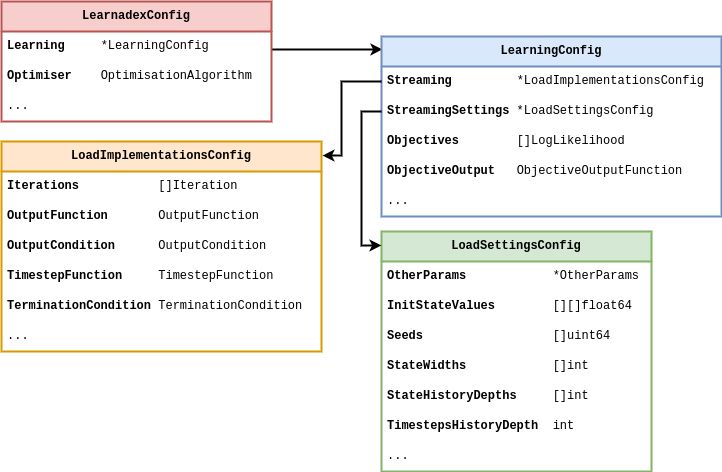
\includegraphics[width=7cm]{images/chapter-3-learnadex-data-types.drawio.png}
\caption{The learning config data type.}
\label{fig:learnadex-data-types-design}
\end{figure}

On the learning side; in order to define a specific objective for each data iterator to compute while the data streams through it, we have abstracted a `log-likelihood' type. Each data iterator is defined as a standard stochadex iteration, hence it can stream data into the learning algorithm from any user-defined source --- e.g., from a file on disk, from a local database instance or maybe via a network socket. In Fig.~\ref{fig:learnadex-data-iterator} below, we provide a schematic of the method calls of (and within) each data iterator.

\textcolor{red}{\begin{itemize}
\item{refactor the code and integrate the reweighting algorithm with Libtorch models for the conditional probabilities --- describe how this is supported}
\item{describe the method calls diagram in more detail --- in particular, point out how it can replace the \texttt{Iteration.Iterate} method which is called when the \texttt{StateIterator} is asked for another iteration from the \texttt{PartitionCoordinator} of the stochadex}
\item{then talk about the optimiser! starting with non-gradient-based: the two packages that are supported out of the box are gonum and eaopt (still need to do gago --- see here: github.com/maxhalford/eaopt) }
\item{also need to then support gradient-based algorithms (like vanilla SGD) by implementing Eq.~(\ref{eq:log-likelihood-reweighting-grad}) for the current basic implementations in the learnadex --- shouldn't be too difficult!}
\item{then talk about the output - talk about the possibilities for output and what the default setting to json logs is for}
\item{could also be written to, e.g., a locally-hosted database server and the best-suited would be a NoSQL document database, e.g., MongoDB~\cite{mongodb}, but building something bespoke and simpler is more aligned with the use-case here and with the principles of this book}
\item{describe the need for log exploration and visualisation and then introduce logsplorer - a REST API for querying the json logs (with basic filtering and selection capabilities but could be extended to more advanced options) and optionally also launches a visualisation React app written in Typescript}
\item{note how this could be scaled to cloud services easily and remotely queried through the logsplorer API and visualised} 
\end{itemize}}

\begin{figure}[h]
\centering
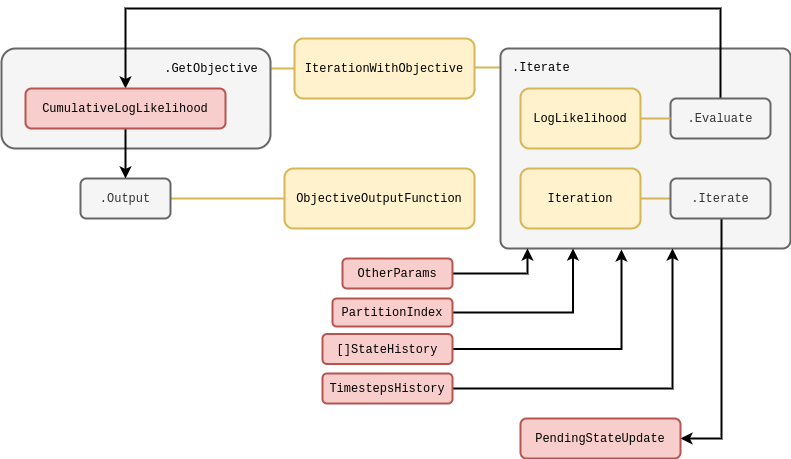
\includegraphics[width=14cm]{images/chapter-3-learnadex-data-iterator.drawio.png}
\caption{A schematic of an iteration with an objective function evaluation.}
\label{fig:learnadex-data-iterator}
\end{figure}

As with the software we wrote for the stochadex, the learnadex main binary executable leverages templating to enable full configurability of all the implementations and settings of Fig.~\ref{fig:learnadex-data-types-design} through passing configs at runtime. Users can alternatively use the learnadex as a library for import, if they desire more control over the code execution. 

\begin{figure}[h]
\centering
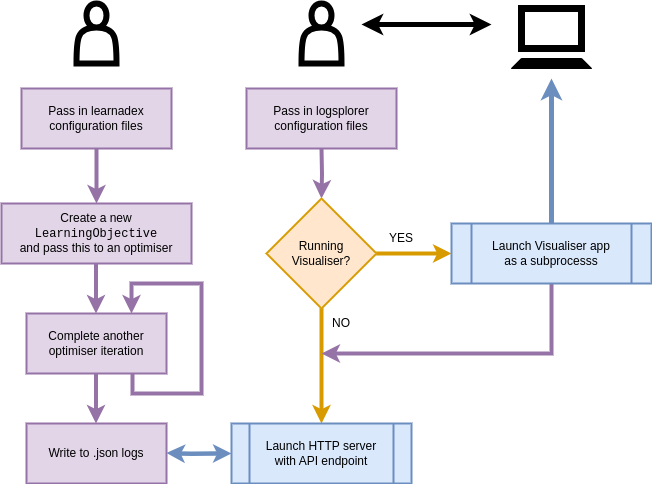
\includegraphics[width=13cm]{images/chapter-3-learnadex-main.drawio.png}
\caption{A diagram of the main learnadex and logsplorer executables.}
\label{fig:learnadex-main}
\end{figure}

\textcolor{red}{Take a step back at this point and consider all the use-cases for the learnadex:
\begin{itemize}
\item{Core functionality is to enable iterative updates to the $P_{\sf t}(X,z)$ distribution at every timestep. There must also be flexibility in how this distribution can represented, i.e., either:
\begin{itemize}
\item{a set of Monte Carlo samples, or}
\item{a set of distribution parameters}
\end{itemize}
}
\item{For Monte Carlo samples, we must also keep the flexibility to use either a BSL or ABC-style data-to-sim comparison in order to facilitate the update}
\item{For distribution parameters, the update can be custom-built by the user with online likelihood-based inference/Bayes estimator methods}
\item{Separate thread context runs of online learning methods using an update method, e.g.,}
\begin{itemize}
\item{Gradient-free batch optimisation with any chosen learning algorithm}
\item{Gradient-based parameter updates}
\item{Arbitrary parameter updates from a different method}
\end{itemize}
\end{itemize}}
    




